%%
%% Copyright 2007, 2008, 2009 Elsevier Ltd
%%
%\pdfoutput=1
%\pdfminorversion=4 % necessary for EES
%
\documentclass[preprint,12pt]{elsarticle}

%% Use the option review to obtain double line spacing
%% \documentclass[authoryear,preprint,review,12pt]{elsarticle}

%% Use the options 1p,twocolumn; 3p; 3p,twocolumn; 5p; or 5p,twocolumn
%% for a journal layout:
%% \documentclass[final,1p,times]{elsarticle}
%% \documentclass[final,1p,times,twocolumn]{elsarticle}
%% \documentclass[final,3p,times]{elsarticle}
%% \documentclass[final,3p,times,twocolumn]{elsarticle}
%% \documentclass[final,5p,times]{elsarticle}
%% \documentclass[final,5p,times,twocolumn]{elsarticle}

\usepackage[hyphens]{url}
\biboptions{sort&compress, square, comma}
\usepackage[breaklinks=true, linkcolor=blue, citecolor=blue, colorlinks=true]{hyperref}
\usepackage{doi}

\usepackage{graphicx}
\usepackage{caption}
\usepackage[font=footnotesize]{subcaption}

\usepackage{bm}
\usepackage{latexsym, amsmath,amssymb}

%% The amssymb package provides various useful mathematical symbols
\newenvironment{spmatrix}[1]
{\def\mysubscript{#1}\mathop\bgroup\begin{pmatrix}}
	{\end{pmatrix}\egroup_{\textstyle\mathstrut\mysubscript}}
\newcommand*{\putunder}[2]{%
	{\mathop{#1}_{\textstyle #2}}%
}
\usepackage{algorithm}
\usepackage{booktabs,multicol}
\usepackage{algorithmic}
\usepackage[textsize=footnotesize]{todonotes}%used for inline todo notes with \todo[]{}

\usepackage{tikz} %used for tikz graphics
\usepackage{standalone}  %used for tikz graphics
\usetikzlibrary{shapes}  %used for tikz graphics

\usepackage{mathtools}
\usepackage[retainorgcmds]{IEEEtrantools}

%better printing of numbers
\usepackage[T1]{fontenc}
\usepackage[english]{babel}
\usepackage{csquotes}
\usepackage{textcomp}

\usepackage{siunitx}
\sisetup{group-separator={,},
     detect-all,
     binary-units,
     list-units = single,
     range-units = single,
     tophrase = --,
     per-mode = symbol-or-fraction,
     separate-uncertainty = true,
     list-final-separator = {, and }
}
\DeclareSIUnit\atm{atm}

% C++ macro
\def\CC{{C\nolinebreak[4]\hspace{-.05em}\raisebox{.4ex}{\footnotesize ++}}}
% derivative macros
\newcommand{ \ddt } [1] { \frac{ \partial #1 }{ \partial t } }
\newcommand{ \ddx } [1] { \frac{ \partial }{ \partial #1 } }
\newcommand{ \dydx } [2] { \frac{ \partial #1 }{ \partial #2 } }
\newcommand{ \ddydxx } [2] { \frac{ \partial^2 #1 }{ \partial #2^2 } }
\newcommand{\pluseq}{\mathrel{{+}{=}}}
\newcommand{\asteq}{\mathrel{{*}{=}}}

\DeclarePairedDelimiter{\Vector}{\lparen}{\rparen}

%figure path
\graphicspath{{./figures/}}

\journal{Computers and Fluids}

\begin{document}

\begin{frontmatter}

%% Title, authors and addresses

%% use the tnoteref command within \title for footnotes;
%% use the tnotetext command for theassociated footnote;
%% use the fnref command within \author or \address for footnotes;
%% use the fntext command for theassociated footnote;
%% use the corref command within \author for corresponding author footnotes;
%% use the cortext command for theassociated footnote;
%% use the ead command for the email address,
%% and the form \ead[url] for the home page:
%% \title{Title\tnoteref{label1}}
%% \tnotetext[label1]{}
%% \author{Name\corref{cor1}\fnref{label2}}
%% \ead{email address}
%% \ead[url]{home page}
%% \fntext[label2]{}
%% \cortext[cor1]{}
%% \address{Address\fnref{label3}}
%% \fntext[label3]{}

\title{GPU-based fluid-structure interaction using immersed boundary methods}

%% use optional labels to link authors explicitly to addresses:
%% \author[label1,label2]{}
%% \address[label1]{}
%% \address[label2]{}

\author[osu]{Christopher S.~Minar}
\author[osu]{Kyle E.~Niemeyer\corref{cor1}}
\ead{Kyle.Niemeyer@oregonstate.edu}

\cortext[cor1]{Corresponding author}
\address[osu]{School of Mechanical, Industrial, and Manufacturing Engineering\\
              Oregon State University, Corvallis, OR 97331-6001, USA
              }


\begin{abstract}
    Engineering applications often require fast, accurate solutions of fluid flow around freely
    moving bodies. The massive parallelism enabled by the graphics processing unit (GPU) architecture
    enables high performance, offering a promising alternative to traditional solver acceleration
    via multicore central processing units (CPU). However, fully harnessing GPU parallelism
    requires specialized algorithms and computing strategies. This work modifies direct-forcing
    immersed boundary methods to model fluid-structure interaction and investigates the performance
    of the methods on GPUs. We verified the solvers using lid-driven cavity flow, impulsively started
    flow over a cylinder, flow over a forced oscillating cylinder, and vortex-induced vibration.
    \todo[inline]{needs more specific results}
\end{abstract}

\begin{keyword}
    GPU \sep computational fluid dynamics \sep immersed boundary method \sep fluid-structure interaction
\end{keyword}

\end{frontmatter}

%% \linenumbers

%% main text
\section{Introduction}
Wave energy converters are seafaring devices that harvest waves to create electrical energy.
In the Atlantic, the sea floor can be shallow enough to use pylons to support devices on the surface.
A wave energy converter can use the relative motion of a buoy rolling in the waves and the anchored pylon to generate electricity.
In the Pacific, the sea floor is too deep to make use of the sea bed.
Instead, some wave energy converters use a large underwater disk called a ``heave plate''.
The purpose of a heave plate is to make as much drag as possible when the buoy tries to pull it up through the water, creating an relatively immobile base substitute for an anchor.
To make wave energy converters cost competitive with established renewable and fossil fuels, they must be optimized to be as efficient as possible.
This paper will discuss the development and characterization cuIBM-FSI~\cite{cuIBM-FSI:v0.1}, a fast fluid flow solver for handling fluid structure interaction with complex bodies.

Graphics processing units (GPUs) have a large theoretical performance for highly parallel problems.
The extensive linear algebra required in computational fluid dynamics presents an enticing opportunity for GPUs.
To achieve a speedup over commercial solvers, cuIBM-FSI performs most calculations using GPUs.

A lot of recent work has focused on writing algorithms to work on GPU-accelerated hybrid clusters, or traditional supercomputers with GPUs available at each node~\cite{xu2014collaborating,liu2016hybrid,norouzi2016new}.
This is sometimes referred to as GPU acceleration.
When there is only one node, such as in a workstation, data transfer times can prohibit efficient simultaneous use of both CPU and GPU.
cuIBM-FSI was forked from cuIBM~\cite{layton2011cuibm}, a GPU-based immersed boundary solver primarily based on the method developed by Taira and Colonius~\cite{Taira:2007jl}.
cuIBM can not handle coupled fluid-structure interaction and produces numerical oscillations when working with moving bodies~\cite{Krishnan:2012jt}.
Improvements to cuIBM include adding fluid-structure interaction and suppressing numerical oscillations by implementing a new fluid solver based on the method presented by Luo et al.~\cite{Luo:2012gx}.

Immersed boundary methods (IBMs) refer to a group of approaches used to simulate fluid flow over complex bodies, representing a body without using a body-fitted mesh.
Immersed boundary method techniques are applicable to a wide range of problems, as reviewed by Mittal and Iaccarino~\cite{Mittal:2005ii} and more recently Sotiropoulos and Yang~\cite{Sotiropoulos:2014gv}.
These techniques are well-suited for simulating flow involving complex, moving bodies because they do not require re-meshing between time steps.
We have implemented two immersed boundary method solvers for operating on, and investigating, graphics processing units designed to handle incompressible fluid--structure interaction problems with rigid bodies.
The methods focused on in this work are both from a popular subgroup of immersed boundary methods known as direct forcing methods \cite{MohdYusof:1997wh, Fadlun:2000fl}.
Direct forcing methods interpolate for velocity at the nodes nearest to the body using the body velocity, eliminating the need to solve for a forcing term while simultaneously enforcing the no-slip condition.

Using a direct forcing method with a moving body can cause numerical oscillations~\cite{Sotiropoulos:2014gv,liao2010simulating,Luo:2012gx}.
This effect is manageable for preset motion, but with a freely moving body the solver can poorly predict body position, fluid values, and forces.
The numerical oscillations are caused by having different solution regimes in the domain, e.g., interpolation near the body and Navier--Stokes everywhere else.
Luo et al.~\cite{Luo:2012gx} suppress the numerical oscillations with a weighting function to transition between the two schemes, removing the discontinuity where the regimes transition.

\section{Numerical methods and Implementation}\label{chapter:Numerical Methods}
The cuIBM-FSI is comprised of two methods based off the work of Luo et al.~\cite{Luo:2012gx}.
For now, it will suffice to refer to these as the external, and embedded methods, leaving their explanations for later.

Both methods start with the two-dimensional, incompressible form of the Navier--Stokes momentum and mass continuity equations:
\begin{align}
\frac{\partial \textbf{u}}{\partial t} + \nabla ( \textbf{uu} ) &= -\nabla p + \nu\nabla^{2}\textbf{u} \label{eq:NavierStokes} \\
\nabla \cdot \textbf{u} &= 0, \label{eq:Continuity} \;.
\end{align}
where $\textbf{u}$ is velocity, $p$ is pressure, and $\nu$ is the (constant) kinematic viscosity.
The fractional-step approach~\cite{Perot1993} is used to solve Equations \eqref{eq:NavierStokes} and \eqref{eq:Continuity}, which breaks up the discretization of the Navier--Stokes equations into three sub-steps.
In the first sub-step, the momentum equations are solved without pressure to  calculate an intermediate velocity:
\begin{equation}\label{eq:Intermediate Velocity}
\hat{\textbf{u}} - \frac{\Delta t}{2}L(\hat{\textbf{u}}) = \textbf{u}^n + \Delta t(\textbf{RHS}^n) \;,
\end{equation}
where $\hat{\textbf{u}}$ is the intermediate velocity, $\Delta t$ is the time step, $L$ is the Laplacian operator, and $\textbf{RHS}$ contains the discretized advection and diffusion terms.
The superscript $n$ represents the current time step, corresponding to time $t^n$.
In time, second-order Adams--Bashforth and Crank--Nicolson methods are used to discretize the advection and diffusion terms, respectively.

In the second sub step, the continuity equation is imposed to approximate the pressure, $p$, resulting in a Poisson equation:
\begin{equation}\label{eq:Poisson}
\nabla^2p^{n+1} = - \frac{\nabla\hat{\textbf{u}}}{\Delta t} \;,
\end{equation}
\newline where $n+1$ indicates the value at the next time step.
Velocity is updated in the last sub step with:
\begin{equation}\label{eq:Projection}
\textbf{u}^{n+1} = \hat{\textbf{u}} - \Delta t\nabla p^{n+1} \;.
\end{equation}

\subsection{GPU implementation strategy}
\label{GPU implementation strategy}
cuIBM-FSI is developed for full GPU operation to improve performance relative to CPU-based algorithms or partial GPU-accelerated approaches which involve significant CPU-GPU communication.
To this end, several overarching strategies have been implemented.

First, all calculations are performed on the GPU, and all data is stored on the GPU.
Although efforts are typically taken to avoid thread divergence when writing code for a GPU, it was found to be favorable to write kernels with occasionally poor thread-parallel performance, i.e., kernels with significant divergence, rather than copying data to the host to do calculations to reduce divergence.
In the cases tested, transferring data back and forth took significantly more time than would be saved by running some operations on a CPU.

Secondly, kernel performance is evaluated compared to the Poisson equation.
Increasing the parallel performance of kernels has little effect on the overall solver performance, because solving the Poisson equation typically takes more than \SI{90}{\percent} of the total computational time.
In addition to non-Poisson kernels being a low overall portion of the run time, the effect of the divergence turns out to be small.
For most kernels, the divergence only occurs in cells near the body which is generally a low percentage of the overall cell count.

The third strategy comes from Layton et al.~\cite{layton2011cuibm}.
When using the CUSP library to perform the multigrid method, creating the preconditioner can take as much time as solving the Poisson equation.
In a moving-body simulation, the preconditioner is normally recalculated each time step, but Layton et al.~\cite{layton2011cuibm} found it possible to skip some time steps without loss of fidelity.
Here, preconditioner is recalculated only if the solution of the previous time step required more than 100 iterations.
The external method does not need the preconditioner to be remade, even when the body is moving, because each node always depends on the same neighbors regardless of the position of the body.

\subsection{Luo et al. method}
To facilitate the discussion of immersed boundary methods, the nomenclature with regards to point identification will be explained here.
The nomenclature is mostly adopted from the work of Luo et al.~\cite{Luo:2012gx} and is similar to Mittal et al.~\cite{Mittal:2005ii}.
There are four types of nodes.
Nodes immediately outside and inside the body are called hybrid nodes and ghost nodes, respectively.
Everything outside of the body that is not a hybrid node is a fluid node.
Everything else (i.e., all nodes inside the body that are not ghost nodes) are solid nodes.
Figure~\ref{fig:node id} shows an example body and grid with labeled nodes.

\begin{figure}[!htb]
	\centering
	\includestandalone[width=0.5\textwidth]{node_id}
	\caption{An example grid with $u$-velocity nodes labeled. Squares mark nodes inside the immersed boundary and circles mark nodes outside the boundary. Solid markers indicate the nearest nodes to the boundary.}
	\label{fig:node id}
\end{figure}

Hybrid nodes are interpolated for using values at the body and nearby fluid nodes.
Ghost nodes have data extrapolated across the body using nearby fluid nodes,in a way that enforces the body's boundary conditions.
Fluid nodes are solved with the Navier--Stokes equations.
The treatment of solid nodes does not affect the solution, but it does affect the computational time and force calculation.
If solid nodes are solved, an arbitrary flow field will develop inside the body.

At the beginning of each time step, nodes are identified using a ray-tracing algorithm (described in O'Rourke~\cite{o1998computational}).
The implementation is based on the CPU implementation from cuIBM~\cite{krishnan2012validation}.
One thread is generated for each node, be it $u$, $v$, or $p$ and this thread performs the following actions to find rays in the $x$ direction.
First, the Lagrangian body nodes are looped through to make segments with their nearest neighbors.
If the top of this segment is above the node and the bottom of the segment is below the node, then the $x$ location of the body at the height of the node is found (open circle in Figure~\ref{fig:node id 1}).
The node is then tested for proximity to the body in the $x$ direction.
To determine what the node is, five $x$-coordinates are used: $x_{i-1}$, $x_{i}$, $x_{i+1}$, $x_{BI}$, and $x_{\text{body center}}$.
Using Figure \ref{fig:node id 1} for example, the body intercept will test as being greater than the body center, greater than $x_{i-1}$, and less than $x_{i}$, which makes $u_{i,j}$ a hybrid node.
\begin{figure}
	\centering
	\includestandalone[width=0.5\textwidth]{node_id_1}
	\caption{To find the hybrid and ghost nodes the position of the body must be translated from the Lagrangian body nodes to the Eulerian grid. The solid line is the real body which is represented by the Lagrangian body nodes (solid circles). The dashed lines are drawn between the body nodes and represent the discretized body.}
	\label{fig:node id 1}
\end{figure}
It is possible for a hybrid or ghost node to be unable to find the body when searching in the $x$ direction, e.g., if the node is above the highest body node.
After the algorithm looks for intersections in the $x$ direction, it searches in the $y$ direction.
In the case where a node is able to find the body in both the $x$ and $y$ directions, the $x$ direction is always chosen.
The $v$-velocity and pressure nodes are found in the same way as described above, but using different coordinates.

After all the points have been tagged, the solid nodes are set to an arbitrary value so they can be easily found later.
This step is not critical for the solution of the Navier--Stokes equations, but is needed for the force calculation, which disregards everything inside the body, and can be convenient when visualizing the solution.

\subsubsection{Weighting}
As the body moves across the background grid, nodes change how they calculate values.
For example a bulk-fluid $u$-velocity node at time step $t^n$ could become hybrid node at time step $t^{n+1}$.
As the node transitions, the intermediate velocity is first calculated by Navier--Stokes (Equation~\eqref{eq:Intermediate Velocity}), then with interpolation (Equation~\eqref{eq:Interpolation}).
Both equations are correct representations for the intermediate velocity, but have different errors, causing the calculated velocities to be slightly different.
This discontinuous change is responsible for numerical oscillations.

In the method proposed by Luo et al.~\cite{Luo:2012gx}, hybrid node values are calculated via both Navier--Stokes and interpolation, and a weighted combination smooths the transition between solutions.
When the hybrid node is close to the body, it will be dominated by the interpolated solution, while a hybrid node far from the body will be dominated by the Navier--Stokes solution.

The weighting scalar $\alpha$ is introduced to the solutions for intermediate velocity and the pressure:
\begin{equation}\label{eq:Weight}
\theta = \left(1-\alpha \right)\theta_{\text{Navier-Stokes}} + \alpha \theta_{\text{Interpolated}}, \;
\end{equation}
where $\theta$ represents either intermediate velocity or pressure.
Transitioning between the Navier--Stokes and interpolated solutions should meet three criteria:
\begin{enumerate}
	\item Hybrid nodes farther from the body should favor the Navier--Stokes solution ($\alpha \rightarrow 0$ as distance $\uparrow$).
	\item Hybrid nodes closer to the body should favor the interpolated solution ($\alpha \rightarrow 1$ as distance $ \rightarrow 0$).
	\item The weighting function should be smooth and continuous as the hybrid node moves away from the body.
\end{enumerate}
To solve for $\alpha$, it is assumed that each hybrid node has at most two neighboring ghost nodes (this will not be true for sharp corners):
\begin{equation}
\alpha = \sqrt{\left(\frac{\Delta_1}{\Delta x}\right)^2 + \left(\frac{\Delta_2}{\Delta y}\right)^2}, \;
\label{eq:Alpha}
\end{equation}
where $\Delta_1$ and $\Delta_2$ correlate to GN$_1$ and GN$_2$, respectively, and $\Delta x$ and $\Delta y$ are the grid spacing in the $x$ and $y$ directions, respectively.
As described by Luo et al.~\cite{Luo:2012gx} and shown in Figure~\ref{fig:Weight}, $\Delta_1$ and $\Delta_2$ are the closest distances between the body and the $x$ and $y$ ghost nodes, respectively.
If the hybrid node only has one neighbor, then $\Delta=0$ for the other direction.
\begin{figure}[!htb]
	\centering
	\includestandalone[width=0.5\textwidth]{alpha_figure}
	\caption{An example grid labeling values needed to calculate $\alpha$ for a $u$-velocity hybrid node. The body intercepts (open circles) are found by projecting from the hybrid or ghost node along the surface normal. $\Delta_1$ and $\Delta_2$ are the distance between the ghost nodes and their respective body intercepts.}
	\label{fig:Weight}
\end{figure}

\subsubsection{Field extrapolation to ghost nodes}

To use the Navier--Stokes equations at hybrid nodes, velocity and pressure must be extrapolated across the body to the ghost nodes using boundary conditions such that the presence of the immersed body is imposed.
No-slip is used for velocity and the pressure boundary condition is approximated by assuming a constant change in pressure along the surface normal.
If the slope of velocity between the hybrid node and the body is assumed to be linear, then the slope can be extrapolated inwards to the ghost node.

Luo et al.~\cite{Luo:2012gx} extrapolated field values across the body using 2D bilinear interpolation.
cuIBM-FSI uses a staggered grid, causing the extrapolation process to have three variations.
The process will be described and shown for $u$-velocity nodes but is the same for $v$ and pressure.
Values are first interpolated for at an image point, represented by triangles in Figure~\ref{fig:Ghost node extrapolation}, outside the body using the surrounding velocities and the boundary condition.
The 2D bilinear interpolation approximates the velocity between four nodes surrounding the image point with Equation~\eqref{eq:Interpolation}.
Each node surrounding the image point is used to set up a system of four equations to solve for the coefficients of Equation~\eqref{eq:Interpolation}, which can then be used to solve for the velocities.
Some of the interpolation nodes are moved to account for the presence of the body.
In Figure~\ref{fig:Ghost node extrapolation} the bottom left corner of each interpolation region is moved to the body intercept point.
\begin{figure}[!htb]
	\centering
	\includestandalone[width=0.5\textwidth]{GN_interp_figure}
	\caption{An example grid showing the relevant nodes for extrapolation of two different types of $u$-velocity ghost nodes.}
	\label{fig:Ghost node extrapolation}
\end{figure}

The ghost nodes, indicated by solid squares, are projected onto the surface to find the body intercept, indicated by the thick open circle.
Body nodes used to track the body's position are not the same as the body intercept and the two are typically not coincident.
If the body has curvature, the body intercept will not fall exactly on the body due to its discrete representation of the body.
The line drawn between the body intercept and ghost node will be perpendicular to the tangent line at the body intercept, i.e., the ghost node is projected along the surface normal.
That line is then mirrored over the surface to find the image point, indicated by the solid triangle.

The rules to determine which values are used to interpolate for the image point are as follows:
If one of the four interpolation nodes is inside the body, as seen in the extrapolation for ghost node 1 in Figure~\ref{fig:Ghost node extrapolation}, then that node is moved to the body intercept and the boundary condition is used.
It is possible for multiple corners to be inside the body.
Any corner inside the body will always be a ghost node and have its own, corresponding body intercept.
All corners inside the body are moved to their corresponding body intercept such that there are always four corners in separate locations to use for the interpolation.
If none of the four velocities are inside the body as seen in the extrapolation for ghost node 2, then the node closest to the body intercept is moved to the body intercept.
To satisfy the no slip condition at the body, a Dirichlet boundary condition equal to the body velocity is used when extrapolating for velocity ghost nodes.
The pressure boundary condition is approximated by forcing the slope of pressure normal to the body surface, $\frac{dp}{dn}$, as constant using Neumann boundary conditions, Equation~\eqref{eq:Neumann}.
Using the relocated corners, a system of equations is set up to solve for the coefficients in Equation~\eqref{eq:Interpolation}.
Pressure nodes on the body use Equation~\eqref{eq:Neumann Node} in the system, which is simply the derivative of Equation~\eqref{eq:Interpolation}:
\begin{align}
\phi (x,y) = a_0 + a_1 x + a_2y + a_3 x y \label{eq:Interpolation} \\
\phi (x,y) = a_1 + a_2 + a_3 (x+y) \label{eq:Neumann Node} \\
\left. \frac{\partial p}{\partial \textbf{n}}\right|_{BI} = \left. -\rho \frac{D\textbf{u}}{Dt}\cdot \hat{\textbf{n}}\right|_{BI},
\label{eq:Neumann}\;.
\end{align}
where $\phi$ is the variable being interpolated ($u$, $v$, or $p$); $a_0$, $a_1$, $a_2$ and $a_3$ are coefficients; $x$ and $y$ give the node location;
$\rho$ is the density; $D\textbf{u}\left/Dt\right.$ is the material derivative; and $\textbf{n}$ is the unit vector normal to the body.
Solving this system on the GPU requires direct inversions of the $4 \times 4$ matrices;
Appendix~\ref{app:inversion} details this procedure.
Once the $a$ coefficients have been found, the velocity at the image point can be calculated with Equation~\eqref{eq:Interpolation} and extrapolated across the surface using Equation~\eqref{eq:Velocity Interpolation} for velocity or ~\eqref{eq:Pressure Interpolation} for pressure:
\begin{align}
\textbf{u}_{GN} &= 2\textbf{u}_{BI} - \textbf{u}_{IP} \label{eq:Velocity Interpolation} \\
p_{GN} &= p_{IP} - \Delta l \left. \frac{\partial p}{\partial \textbf{n}}\right|_{BI}, \; \label{eq:Pressure Interpolation}
\end{align}
where the subscripts GN, BI, and IP indicate ghost nodes, body intercept, and image point, and $\Delta l$ is the distance from ghost node to image point.

\subsubsection{Interpolation to hybrid nodes}
\label{Sec:Interpolation}

Interpolating for the field value at the hybrid node is largely the same as the ghost nodes procedure previously.
The body intercept is once again found by projecting the hybrid node along the surface normal.
The image point is not used in the same way as the ghost node image point.
If a given body intercept is located at $(x_{BI},y_{BI})$ and its hybrid node is located at $(x_{BI}+\Delta x,y_{BI}+\Delta y)$, the corresponding image point is located at $(x_{BI}+2\Delta x,y_{BI}+2\Delta y)$ as shown in Figure~\ref{fig:Interpolate}.
For a hybrid node, an image points purpose is only to locate the four interpolation nodes, one of which will always be the corresponding hybrid node.
The interpolation node coincident with the hybrid node is moved to the body intercept and the appropriate boundary condition for velocity or pressure is applied.
Once Equation~\eqref{eq:Interpolation} is solved, the hybrid node is interpolated for.

\begin{figure}[!htb]
	\centering
	\includestandalone[width=0.5\textwidth]{HN_interp_figure}
	\caption{An example grid showing the relevant nodes for interpolation to a $u$-velocity hybrid node.}
	\label{fig:Interpolate}
\end{figure}

\subsubsection{External method}
\label{sec:ID external}
cuIBM-FSI has two methods based off the approach given by Luo et al.~\cite{Luo:2012gx}.
The key difference between the two approaches is when the extrapolation and interpolation takes place.
The ``embedded'' method performs  interpolations, extrapolations, and weighting inside of the linear algebra solutions for the intermediate velocity and pressure.
All of the extrapolation and interpolation happens inside of the linear algebra steps.
Field values will solved by plugging Equations~\eqref{eq:Intermediate Velocity} or \eqref{eq:Poisson} and \eqref{eq:Interpolation} into Equation~\eqref{eq:Weight}.
The discretization of these can be seen in Section \ref{sec:ID embedded}.
The ``external'' method moves the interpolation and extrapolation outside of the linear algebra.
Separating the extrapolation, interpolation, and linear algebra steps causes each one to not have access to the most updated information when being calculated because they all depend on each other.
Simplifying the linear algebra this way reduces the computational time at the cost of reduced accuracy and increased numerical oscillation.

Two key implementation details distinguish cuIBM-FSI from Luo et al.~\cite{Luo:2012gx}.
Firstly, Luo et al.~did not use a staggered grid.
Secondly, Luo et al.~used Crank--Nicholson to discretize both the advection and diffusion terms, whereas cuIBM-FSI uses Adams--Bashforth for the advection terms.

Before a value is used by the fractional-step calculations, it is calculated at the hybrid and ghost nodes.
For example, the equation for intermediate velocity, Equations~\eqref{eq:Intermediate Velocity}, depends on the velocity field, so $u$ and $v$ are interpolated for at the hybrid nodes and extrapolated for at the ghost nodes before the right-hand side matrix is calculated.
The following sequence is set up such that a value is interpolated or extrapolated just before it is needed for the subsequent step:

\begin{enumerate}
	\item Identify all nodes as hybrid, ghost, fluid, or solid.
	\item Extrapolate $u$ and $v$-velocity values to ghost nodes.
	\item Interpolate for $u$ and $v$-velocities at hybrid nodes.
	\item Calculate the right-hand side terms for the intermediate velocity solution.
	\item Solve for intermediate velocity.
	\item Weight the two intermediate velocity solutions.
	\item Extrapolate intermediate velocities to ghost nodes.
	\item Calculate the right-hand side terms for the Poisson equation.
	\item Solve the Poisson equation.
	\item Interpolate for pressure at hybrid nodes.
	\item Weight the two pressure solutions.
	\item Extrapolate pressure to ghost nodes.
	\item Update velocity.
	\item Advance time.
\end{enumerate}

\subsubsection{Embedded interpolation method}
\label{sec:ID embedded}
In the intermediate velocity sub-step, the right hand side terms are first calculated as if no body was present.
The weighting coefficients and part of the interpolation can be calculated prior to the linear algebra as they are only dependent on the geometry, not velocity or pressure.
The equations for bilinear interpolation, Equation \eqref{eq:Interpolation}, and interpolating to the ghost node, Equations \eqref{eq:Velocity Interpolation} or \eqref{eq:Pressure Interpolation}, are combined then rearranged to separate field value terms.
A similar operation happens for the hybrid nodes.
To illustrate the process of separating these variables, $u$ is plugged in for $\phi$ in Equation~\eqref{eq:ID reorganized interpolation}:
\begin{equation}
u(x,y) = a_0 + a_1x +a_2y+a_3xy.
\end{equation}
Each bilinear interpolation requires four data points to solve as discussed above.
They will be labeled roughly according to their cardinal direction to the interpolation location.
The resulting system of equations is laid out below in \eqref{eq:interp_matrix}.
\begin{gather}
\putunder{
	\begin{bmatrix}
	1&x_{sw}&y_{sw}&x_{sw}y_{sw}\\
	1&x_{se}&y_{se}&x_{se}y_{se}\\
	1&x_{nw}&y_{nw}&x_{nw}y_{nw}\\
	1&x_{ne}&y_{ne}&x_{ne}y_{ne}
	\end{bmatrix}
}{\textbf{A}}
\putunder{
	\begin{bmatrix}
	a_0\\
	a_1\\
	a_2\\
	a_3
	\end{bmatrix}
}{\textbf{a}\vphantom{A}}
=
\putunder{
	\begin{bmatrix}
	u_{sw}\\
	u_{se}\\
	u_{nw}\\
	u_{ne}
	\end{bmatrix}
}{\textbf{u}\vphantom{A}}.
\label{eq:interp_matrix}
\end{gather}
Equation~\eqref{eq:Ainverse} gives the exact inverse of matrix $\textbf{A}$:
\begin{align}
\textbf{A}^{-1} = \frac{\textbf{B}}{\det{\textbf{A}}}
\label{eq:Ainverse}\\
\textbf{a}=\textbf{A}^{-1}\textbf{u}.\;\label{eq:acoef}
\end{align}
Matrix $\textbf{B}$ is based on the values of $\textbf{A}$.
The inverse is used to solve for the $\textbf{a}$ coefficients, Equation \eqref{eq:acoef}.
The external method stops here because all the $u$ values are considered known.
The embedded method moves, rearranges, and combines with the ghost node interpolation to become Equation~\eqref{eq:ID reorganized interpolation}:

\begin{equation}
u_{GN} = 2u_{BI} + C_{nw}u_{nw} + C_{ne}u_{ne} + C_{sw}u_{sw} + C_{se}u_{se}\label{eq:ID reorganized interpolation}
\end{equation}
The array $C$ holds the velocity coefficients resulting from \eqref{eq:acoef} being manipulated.
Subscripts indicate the row and column of the matrix.
The calculation of $C$, Equation \eqref{eq:ucoef 1}, is the portion of the bilinear interpolation that is performed before the linear algebra step:
\begin{gather}
\begin{bmatrix}
C_{sw}\\
C_{se}\\
C_{nw}\\
C_{ne}
\end{bmatrix}
=
\begin{bmatrix}
b_{11}+b_{21}x_{IP}+b_{31}y_{IP}+b_{41}x_{IP}y_{IP}\\
b_{12}+b_{22}x_{IP}+b_{32}y_{IP}+b_{42}x_{IP}y_{IP}\\
b_{13}+b_{23}x_{IP}+b_{33}y_{IP}+b_{43}x_{IP}y_{IP}\\
b_{14}+b_{24}x_{IP}+b_{34}y_{IP}+b_{44}x_{IP}y_{IP}
\end{bmatrix}
/\det{(A)}
\label{eq:ucoef 1}
\end{gather}

Before the left-hand side matrix can be calculated, the number of values in the sparse matrix must be found because the hybrid nodes now have a larger stencil than normal.
Figure \ref{fig:ID combined stencil}a shows how the ghost node stencils can be modified.
\begin{figure}[!htb]
	\centering
	\begin{subfigure}{0.5\textwidth}
		\includestandalone[width=\linewidth]{combined_stencil}
		\caption{Stencil modification for ghost nodes. Ghost node 1 has a stencil that only uses four nodes and ghost node 2 has a stencil that uses five.}
	\end{subfigure}

	\begin{subfigure}{0.5\textwidth}
		\includestandalone[width=\linewidth]{combined_stencil_2}
		\caption{The combination of Navier--Stokes (bold lines) and interpolation (shaded section) stencils.}
	\end{subfigure}
	\caption{The stencils of the left-hand-side matrices change when interpolating inside the linear algebra step.}
	\label{fig:ID combined stencil}
\end{figure}
Ghost node 1, in the upper left, only uses four nodes indicated by the open circles.
In a situation where a stencil is smaller than five nodes, an additional node that is not being used is added with a coefficient of zero (this is done because CUSP COO matrices are initialized with a specified number of non-zero nodes).
When initialized, all the values are set at (0,0,0), where the zeros represent the row, column, and value of a given non-zero entry.
If the CUSP multi-grid solver encounters multiple (0,0,0) entries, it will fail to converge upon a solution.
It is easier to add a zero value than to restructure the matrix to not have a value.
Ghost node two, which depends on the nodes marked with open squares, does not need any special treatment because it uses five nodes.

Figure \ref{fig:ID combined stencil} shows the stencil for hybrid nodes, with two overlapping stencils.
The interpolation stencil is shown by the shaded region and depends on the nodes marked with circles.
The Navier--Stokes stencil is marked with the solid black lines and open squares.
Combining the two into a hybrid stencil results in six entries to the sparse matrix.
As the left-hand side matrix is being built, the algorithm will place five of the six nodes in their allocated memory locations.
To place the last node, each hybrid node is counted and labeled from left to right, top to bottom.
Extra memory is allocated to the end of the sparse matrix arrays, with one additional spot for each counted hybrid node.
The sixth entry to sparse matrix is placed at the end of the normal amount of entries to the sparse matrix plus the count of the hybrid nodes.

After the left-hand side matrix is made, it is sorted by row and column using a built-in CUSP function and the preconditioners are rebuilt.
The CUSP solvers are optimized to operate on a sorted matrix and would sometimes fail to converge due to out of order values at the end of the arrays.
During the calculation of the LHS matrix, the modifications to the right hand side matrix are stored in two values.
The first one is a multiplier for the original RHS matrix and the second is added to that value.
This makes it possible to multiply the original value by the Navier--Stokes, weight then add the interpolated weight.
Finally, $\hat{\textbf{u}}$ is calculated using CUSP.

The implementation of the embedded Poisson equation is the same as outlined above.


%%%%%%%%%%%%%%%%%%%%%%%%%%%%%%%%%%%%%%%%%%%%%%%%%%%%%%%%%%%%%%%%%%%%%%%%%%%%%%%%
\section{Verification and validation}
\label{chapter:Validation}

Both methods are tested using several well studies simulations.
The first simulation tests the solvers ability to handle a body with prescribed motion.
In this test, a cylinder has a set sinusoidal motion in an initially stagnant flow.
The second simulation features an impulsively started cylinder, with a set sinusoidal motion.
Both of these tests look at the force calculation for a moving body and help quantify the numerical oscillation caused by direct forcing.
The last simulation is called vortex-induced vibration (VIV) and tests the solvers' ability to accurately predict body location, velocity, and force when the body motion is not prescribed.

\subsection{Flow driven by in-line oscillating cylinder}
\label{sec:Oscillating Cylinder in no Flow}

Liao et al.~\cite{liao2010simulating} used an in-line oscillating cylinder with initial velocities
and Dirichlet boundary conditions of zero to demonstrate numerical oscillation suppression.
Here, we validate the results of Liao et al.~\cite{liao2010simulating} and cuIBM-FSI
against the experimental data of D\"{u}tsch et al.~\cite{dutsch1998low}.
The equations that govern cylinder motion, \eqref{eq:cylinder position2} and \eqref{eq:cylinder velocity2}, are
the same form as above but with a period, maximum velocity, and position of 1, 1, and $1/2\pi$:
\begin{align}
x(t) &= \frac{-1}{2\pi} \sin(2\pi t) \quad \text{and} \label{eq:cylinder position2}\\
u(t) &= -\cos(2\pi t) \;. \label{eq:cylinder velocity2}
\end{align}
The cylinder diameter, 0.2, matches that of Liao et al.~\cite{liao2010simulating}.
These values give the simulation a Reynolds number of 100 and Keulegan--Carpenter (KC) number of 5.
The KC number is a non-dimensional quantity representing the importance of drag and
inertial forces on an oscillating body, calculated with Equation~\eqref{eq:KC}:
\begin{equation}
\text{KC} = \frac{U_\text{max}}{fD} \label{eq:KC} \;,
\end{equation}
where $f$ is the oscillation frequency.
The domain spans $\pm$ 5.5 in $x$ and $\pm$ 3.5 in $y$, and has a fine, uniform grid
spacing of $\Delta x = \Delta y = 0.005$ from $(-0.4,-0.2)$ to $(0.4,0.2)$.
Figure \ref{fig:staticInit} shows the force during the first period versus the steady-state
experimental data of D\"{u}tsch et al.~\cite{dutsch1998low}.
Figure \ref{fig:staticSteady} shows the steady state drag.
The embedded interpolation method suppresses the oscillations more effectively than the external method.
It also better predicts the maximum peak drag force, with around \SI{15}{\percent}
error compared with the experimental data.
\begin{figure}[htbp]
    \centering
    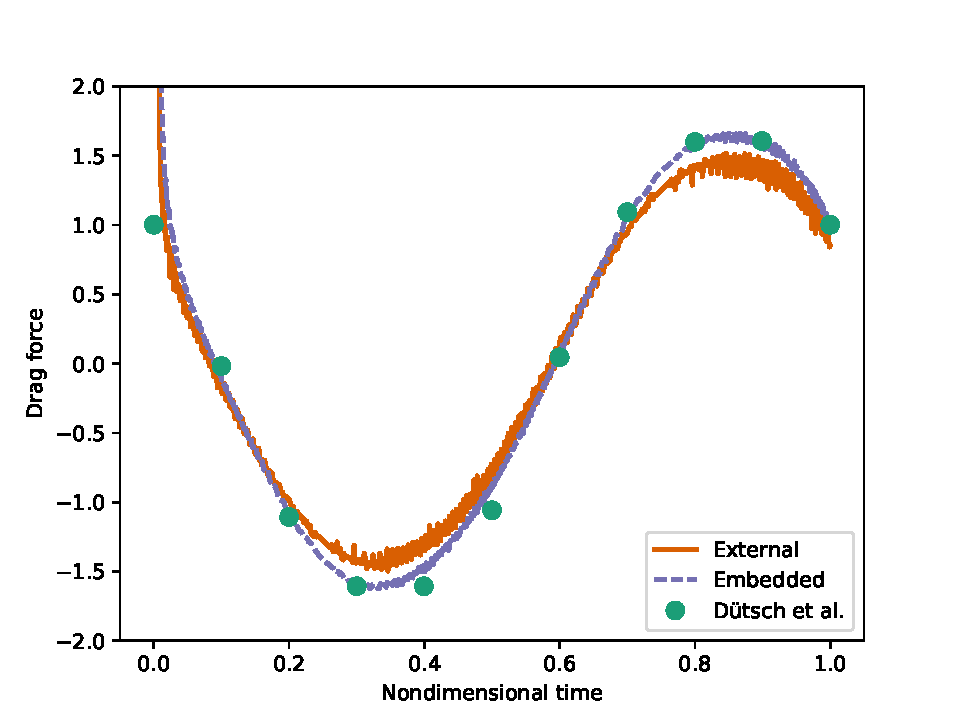
\includegraphics[width=0.75\linewidth]{static_init.pdf}
    \caption{Drag force over the first period for an in-line oscillating cylinder flow
    calculated with the external and embedded interpolation methods, compared with the
    steady-state results of D\"{u}tsch et al.~\cite{dutsch1998low} for KC=5 and Re=100.
    }
    \label{fig:staticInit}
\end{figure}

\begin{figure}[htbp]
    \centering
    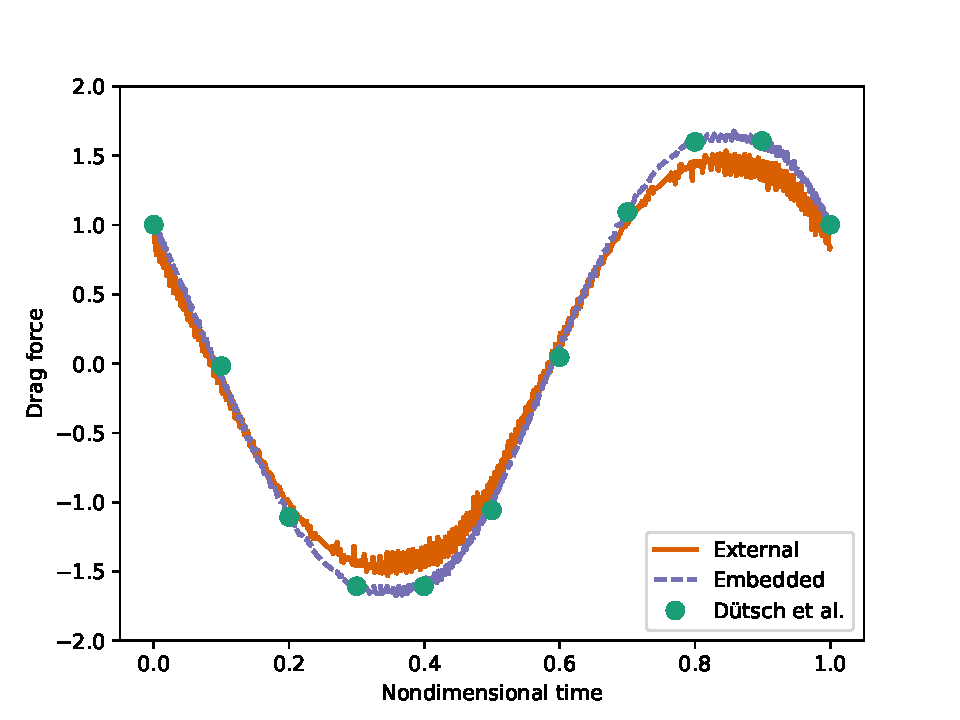
\includegraphics[width=0.75\linewidth]{static_ss.pdf}
    \caption{Drag force over a steady-state period for in-line oscillating cylinder flow
    calculated with the external and embedded interpolation methods, compared with
    the results of D\"{u}tsch et al.~\cite{dutsch1998low} for KC=5 and Re=100.
    }
    \label{fig:staticSteady}
\end{figure}

Figure~\ref{fig:KC 10} shows the validation against D\"{u}tsch et al.~\cite{dutsch1998low}
for a Reynolds number of 200 and KC of 10, during the 14th period.
D\"{u}tsch et al.\ compared drag forces for various cycles into the low 100s.
Re and KC can both be doubled by doubling the maximum velocity of the body, which can
be done by multiplying Equation~\eqref{eq:cylinder velocity2} by two and integrating to
obtain a new position equation. Once again, the embedded method suppresses oscillations
better than the external method, but both reasonably predict the drag force.
\begin{figure}[htbp]
    \centering
    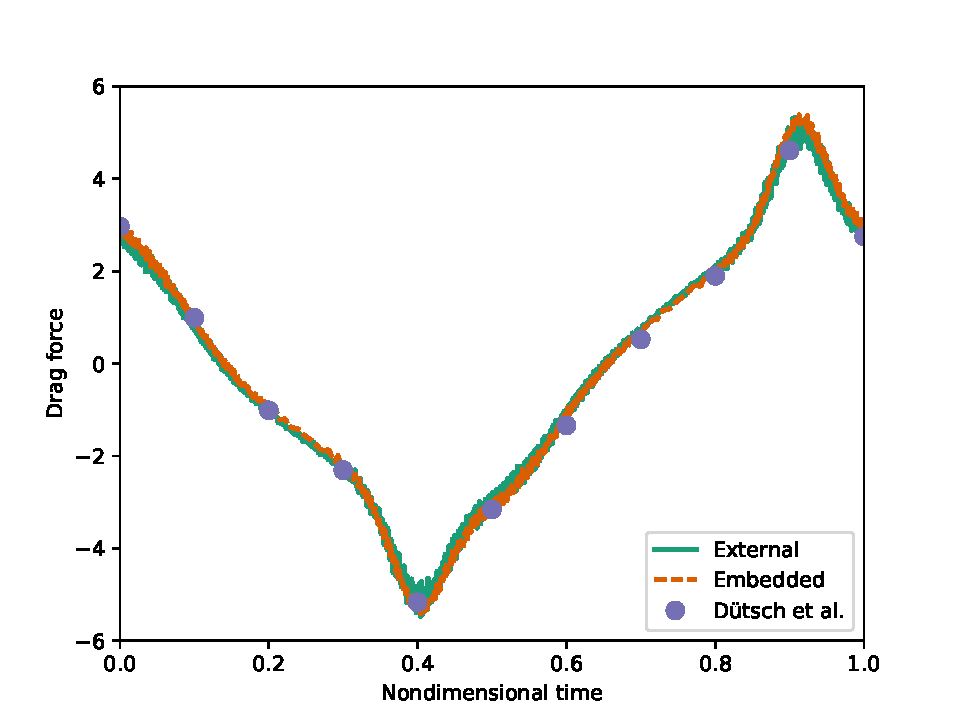
\includegraphics[width=0.75\linewidth]{static_kc10.pdf}
    \caption{Drag force over the 14th period for in-line oscillating cylinder flow
    calculated with the external and embedded interpolation methods,
    compared with D\"{u}tsch et al.~\cite{dutsch1998low} for KC=10 and Re=200.}
    \label{fig:KC 10}
\end{figure}


\subsection{Impulsively started oscillating cylinder}
\label{sec:osccylinder}

The impulsively started oscillating cylinder is a simulation used by Luo et al.~\cite{Luo:2012gx}
to demonstrate and compare the magnitude numerical oscillations between different immersed boundary methods.
An ``impulsively started'' simulation sets the initial conditions to mimic a body being struck by a hammer.
In the first few time steps, a large shear stress on the body will cause high drag,
which rapidly dissipates as the boundary layer develops. To simulate an impulsively started
cylinder, an initial $u$-velocity of one is set over the entire fluid domain.
The left, top, and bottom boundaries use Dirichlet $u$ and $v$ conditions with values of
one and zero forming an inlet and two free stream boundaries, respectively.
A convective boundary condition is used at the exit.\todo{clarify convective BC}{}
The grid is uniformly spaced in the area immediately around the immersed body,
which spans $(-2,-2)$ to $(2,2)$. The cells stretch moving away from the center
until reaching the domain edge at $\pm$ 15.

The cylinder oscillates along the horizontal centerline according to
\begin{align}
    x(t) &= -0.25 \cos(0.4\pi t) \quad \text{and} \label{eq:cylinder position}\\
    u(t) &= 0.1\pi \sin(0.4\pi t) \;. \label{eq:cylinder velocity}
\end{align}
The resulting period, maximum velocity, and position are 5, $\pi/10$, and 0.25, respectively.
Figure~\ref{fig:osccylinder} compares the numerical oscillations observed in drag vs.~time
for the external and embedded methods. The uniform section is discretized into a $64 \times 64$ grid
for the first row and $ 128 \times 128$ grid for last three rows row for $h$ (center
grid spacing) values of 0.0625 and 0.03125. The maximum CFL numbers by row are
approximately \numlist{0.35; 0.35; 0.7; 1.0}.
\begin{figure*}[htbp]
    \centering
    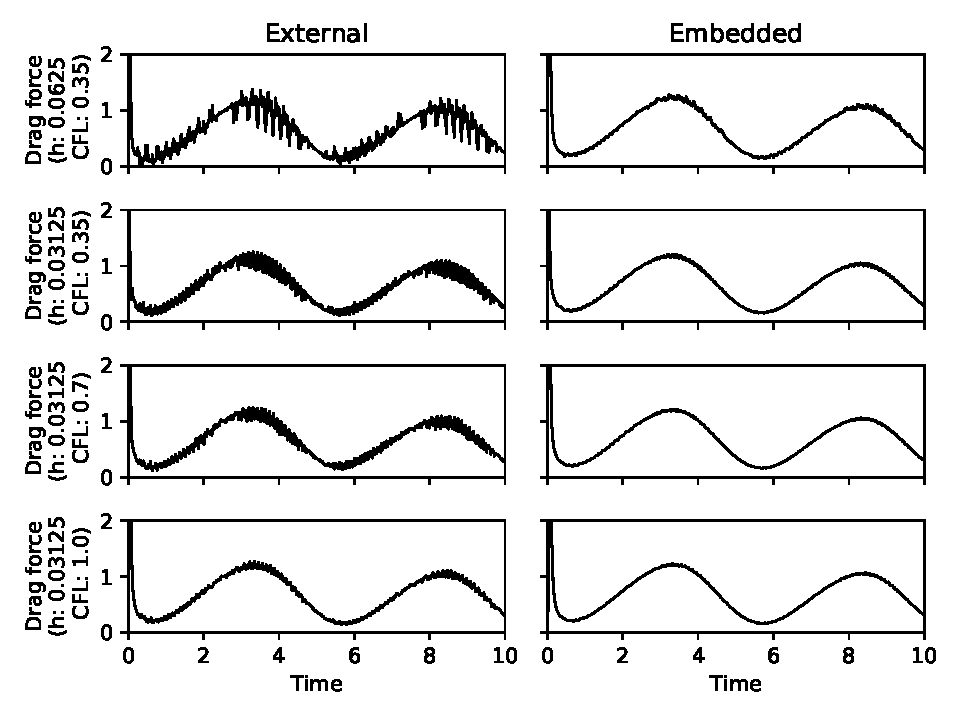
\includegraphics[width=\textwidth]{osc_cylinder}
    \caption{Drag force for flow over an in-line oscillating cylinder. The left
    and right columns show the external and embedded interpolation methods, respectively.
    The four rows show cases with maximum CFL numbers of \numlist{0.35; 0.35; 0.7; 1.0},
    respectively, and a middle grid spacing of \numlist{0.0625; 0.03125; 0.03125; 0.03125}.}
    \label{fig:osccylinder}
\end{figure*}

Both methods increasingly suppress the magnitude of the oscillations with decreasing grid size.
The frequency of the oscillations is also reduced by increasing the maximum CFL number.
This effect is more easily seen in the left column.
The embedded method, as expected, more effectively suppresses oscillations because
it uses updated information for its interpolations, extrapolations, and weighting.
The bottom row of figures show that both methods only suppress the oscillations,
rather than eliminate them entirely. In spite of the oscillations, similar maximum
force values can be obtained from all eight plots.

\subsection{Vortex-induced vibration}
\label{sec:viv}

The vortex-induced vibration simulation tests the solvers' abilities to predict the
position of a freely moving body in coupled fluid-structure interaction.
The two-dimensional domain is the same as the impulsively started cylinder simulation,
except the uniform grid region ranges from $(-1.5, -1.5)$ to $(1.5, 1.5)$.
An immersed two-dimensional cylinder (i.e., a circle) starts at the origin with
no initial velocity. The body is free to move in the $y$ direction but fixed in the
$x$ and mounted to a notional spring. The Reynolds number is set to a range where
the cylinder sheds oscillating vortices---in this case Re=150.
This, combined with the spring, causes the body to establish steady-state sinusoidal motion
for which the amplitude can be verified against literature results.
Following the work of Borazjani et al.~\cite{borazjani2008curvilinear}, the mass-spring
damper system Eq.~\eqref{eq:masspring} that governs the body's movement is
\begin{equation}
    M \ddydxx{Y}{t} + C \ddt{Y} + KY = F_y \;, \label{eq:masspring}
\end{equation}
where $Y$ is the center coordinate of the body, $M$ is the mass, $C$ is the damping factor,
$K$ is the spring stiffness, and $F_y$ is the total fluid force on the body in the $y$ direction.
The natural frequency and critical damping are respectively given by
\begin{align}
    \omega &= 2\pi f = \sqrt{\frac{K}{M}} \quad \text{and} \label{eq:nf}\\
    C_{cr} &= 2\sqrt{MK} = 2K\omega \;. \label{eq:cd}
\end{align}
Equation~\eqref{eq:masspring} can then be non-dimensionalized to
\begin{equation}
    \frac{\partial^2 Y}{\partial t^2}+4\pi \zeta\frac{1}{U_{red}}\frac{\partial Y}{\partial t}
     + 4\pi^2\frac{1}{U_{red}^2}Y=\frac{1}{2M_{red}}C_Y \;,
     \label{eq:ndmasspring}
\end{equation}
where the non-dimensional coefficients are the damping coefficient $\zeta=\frac{C}{C_{cr}}$,
reduced velocity $U_{red}=\frac{U}{fD}$, reduced mass $M_{red}=\frac{M}{\rho D^2}$,
and force coefficient $C_Y=\frac{2F_Y}{\rho U^2 D}$. Varying the parameters Re, $\zeta$,
$M_{red}$, and $U_{red}$ changes the resulting steady-state amplitude.
In vortex-induced vibration there is a ``lock-in'' phenomenon that occurs when
Re=150, $\zeta$=0, $M_{red}$=2, and $U_{red}$ is varied between \numrange{3}{8}.
At either extreme for $U_{red}$, the steady-state amplitude will be small, while
values in between will lead to much larger steady-state amplitudes.

Body position can be updated using two ways: loose and strong coupling~\cite{Sotiropoulos:2014gv}.
Loose coupling comes from an explicit discretization of Equation~\eqref{eq:ndmasspring}.
A time step using loose coupling proceeds as follows:
\begin{enumerate}
    \item Solve for field values at $t^{n+1}$ using the Navier--Stokes equations.
    \item Calculate body forces.
    \item Move body using
\end{enumerate}
\begin{align}
v^{n+1} &= v^n-\frac{\Delta t\pi^24}{U_{red}^2}\left(y^n+\frac{\Delta tv^n}{2}\right) + \frac{\Delta tC_Y}{\left(2M_{red}\right)\left(1+\frac{4\Delta t^2\pi^2}{U_{red}^2}\right)} \label{eq:lc1} \\
y^{n+1} &= y^n +\frac{\Delta t\left(v^{n+1}+v^n\right)}{2}\; \label{eq:lc2}
\end{align}

Equation~\eqref{eq:ndmasspring} can also be discretized implicitly to achieve strong coupling.
A strong coupling time step repeatedly calculates the field values and body
kinetics/kinematics until reaching a converged solution.
As this causes the Poisson equation to be solved multiple times for each time step,
strong coupling is a significantly more computationally expensive method:
\begin{enumerate}
    \item Solve for field values at sub step $t^{k+1}$ using the Navier--Stokes equations.
    \item Calculate body forces
    \item Move body using Equations \eqref{eq:lc1} and
    \begin{equation}
        y^{k+1} = \alpha \left(y^n+\frac{\Delta t\left(v^{k+1}+v^n\right)}{2}\right) +\left(1-\alpha\right)y^k \;,
        \label{eq:sc}
    \end{equation}
    where $\alpha$ is a relaxation value.
    \item If $|Y^{k+1}-Y^k| \approx 0$, advance time; otherwise advance sub step.
\end{enumerate}

Figure~\ref{fig:viv_combine} shows the maximum amplitude of six vortex-induced
vibration simulations as calculated by external loose coupling, external strong coupling,
embedded loose coupling, and embedded strong coupling.\todo{what six?}{}
Results are verified against results from the curvilinear immersed boundary method of Borazjani
et al.~\cite{borazjani2008curvilinear} and the unstructured finite-element approach
of Ahn and Kallinderis~\cite{ahn2006strongly}.
All four configurations used to simulate the vortex-induced vibration phenomena
(i.e., embedded/external and loose/strong coupling) predict the maximum steady state
amplitude accurately, although the external method exhibits noticeable oscillations
of similar magnitude to those shown for the impulsively started oscillating cylinder.
The main difference between the external and embedded method is the wall-clock time
taken to run each, with the embedded method taking nearly an order of magnitude more
than the external method.
\begin{figure*}
    \centering
    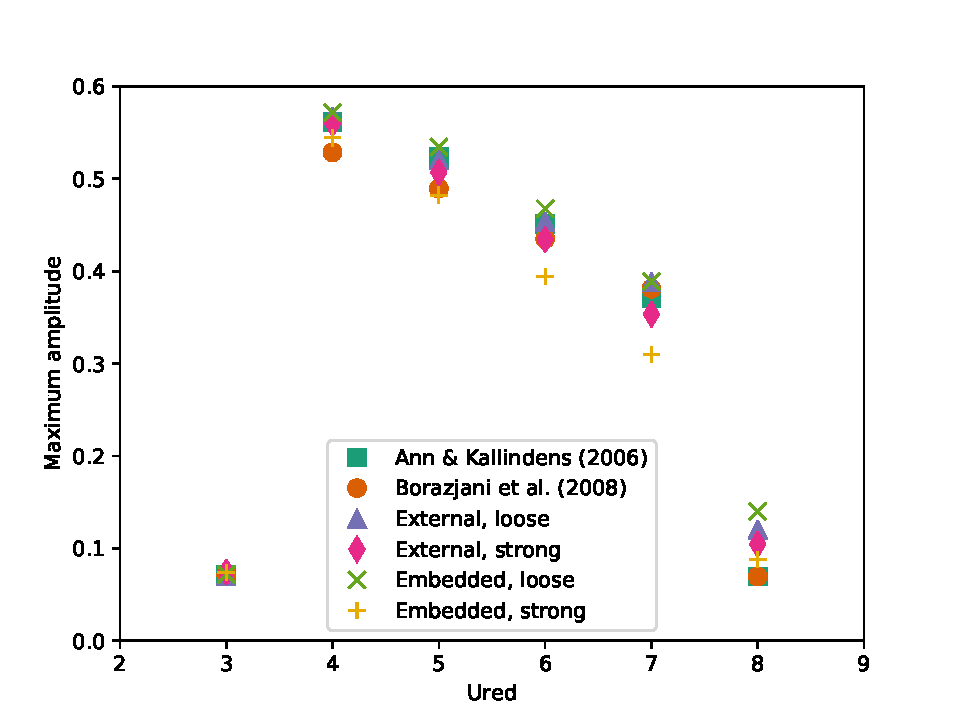
\includegraphics[width=\textwidth]{VIV_combine}
    \caption{Maximum cylinder amplitude in the lock-in region as computed with the
    external and embedded methods using loose and strong coupling.}
    \label{fig:viv_combine}
\end{figure*}

%%%%%%%%%%%%%%%%%%%%%%%%%%%%%%%%%%%%%%%%%%%%%%%%%%%%%%%%%%%%%%%%%%%%%%%%%%%%%%%%
\section{Solver characterization}
\label{chapter:error}

This section will evaluate the methods used in terms of error norms, order of accuracy,
and performance scaling.

\todo[inline]{move description of methods here?}

\subsection{Error norms for impulsively started cylinder flow}

Figure~\ref{fig:error norm} shows the $L_1$, $L_2$, and $L_\infty$ error norms for
the both immersed boundary methods tested using an immobile cylinder.
The $L_1$, $L_2$, and $L_\infty$ error norms are calculated using
\begin{align}
    L_1 &= \sum_{i} \left|u_{\text{fine}, i}-u_{\text{coarse},i}\right| \;, \label{eq:L1 error norm} \\
    L_2 &= \sqrt{\sum_{i} \left(u_{\text{fine}, i}-u_{\text{coarse},i}\right)^2} \;, \text{ and} \label{eq:L2 error norm} \\
    L_{\infty} &= \text{max}_i\left(u_{\text{fine}, i}-u_{\text{coarse},i}\right) \;, \label{eq:Linf error norm}
\end{align}
where $ u_{\text{fine}, i} $ and $u_{\text{coarse}, i}$ are the $x$ velocities at the $i$th grid point
for the finest grid and a particular coarse grid, respectively.\todo{add information about grid sizes considered}{}
The $L_1$ error norm is the sum of all the error in every cell.
$L_2$ is the square root of the sum of the squared errors. The error in each cell is less than one,
so the $L_2$ error norm is several orders of magnitude lower than the $L_1$.
$L_\infty$ is the most intuitive of the error norms: the largest difference between the
fine and coarse grids.
The coarsest grid produces an $L_\infty$ value of 0.2, corresponding to a maximum velocity
around one and a half, for a relative error of about \SI{13}{\percent} (compared with
\SI{3}{\percent} for the finest grid. As the grid size decreases and the cell count
increases, the most accurate solver will have the smallest slope.\todo{clarify}{}
The external method exhibits lower error norms for all measures.

\begin{figure}[htbp]
    \centering
    \begin{subfigure}{0.5\textwidth}
        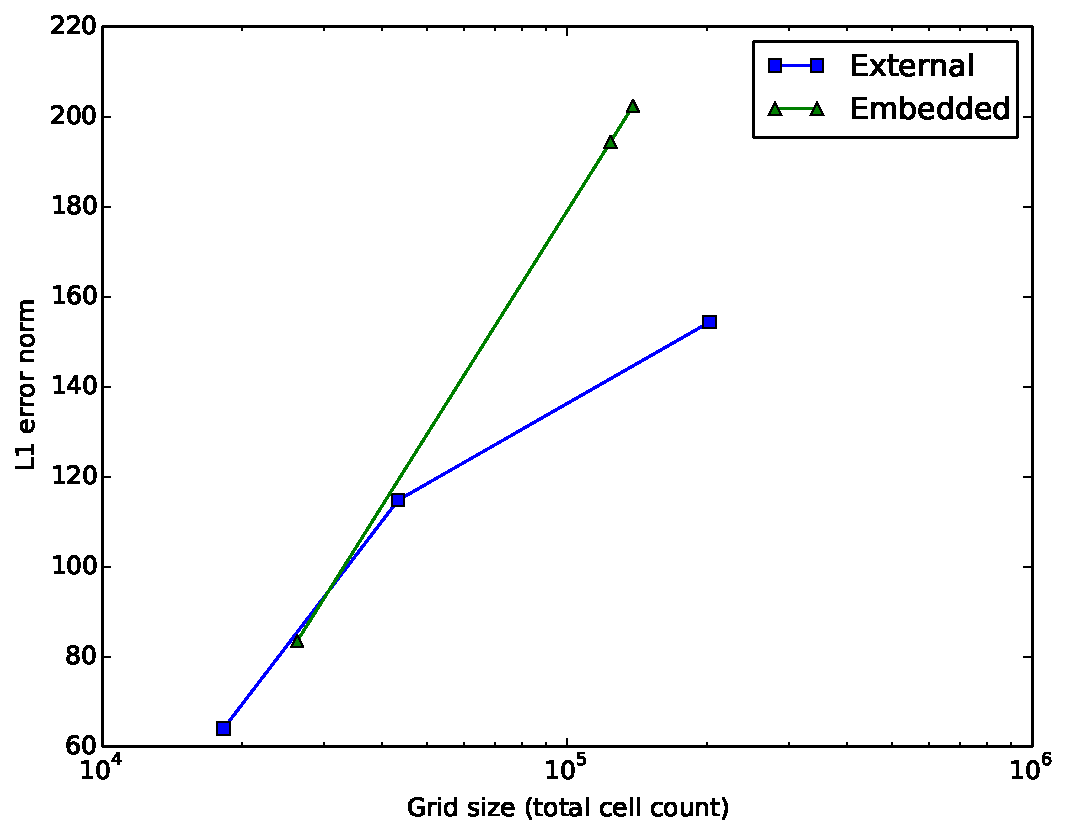
\includegraphics[width=\linewidth]{L1_error_norm}
        \caption{$L_1$ error norm.}
    \end{subfigure}

    \begin{subfigure}{0.5\textwidth}
        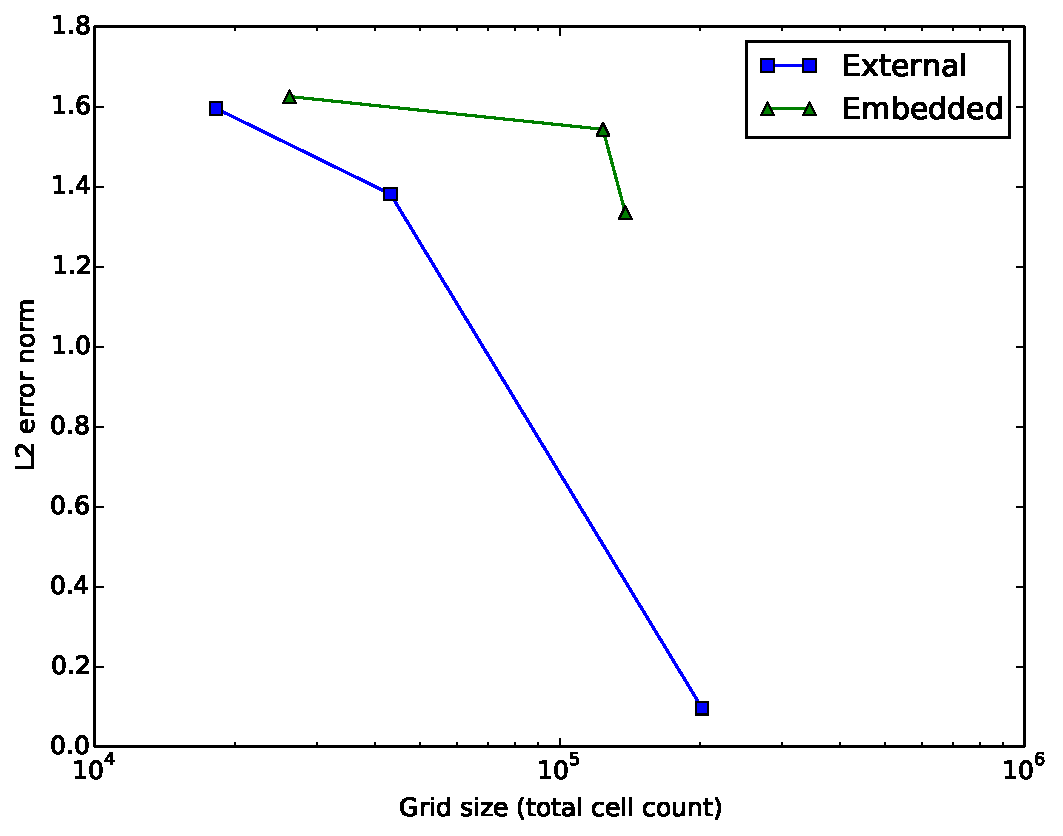
\includegraphics[width=\linewidth]{L2_error_norm}
        \caption{$L_2$ error norm.}
    \end{subfigure}

    \begin{subfigure}{0.5\textwidth}
        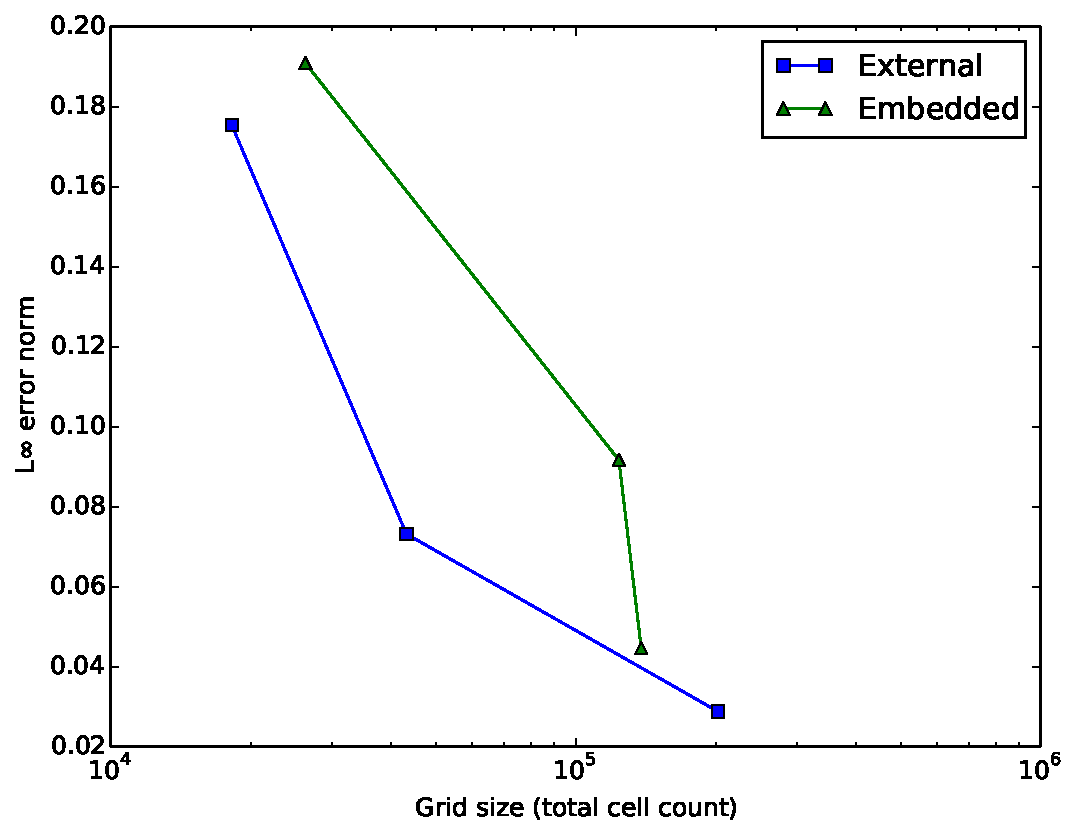
\includegraphics[width=\linewidth]{Linf_error_norm}
        \caption{L$_\infty$ error norm.}
    \end{subfigure}
    \caption{$L_1$, $L_2$, and $L_\infty$ error norms for impulsively started cylinder simulations,
    using the external and embedded interpolation methods.
    }
    \label{fig:error norm}
\end{figure}

\subsection{Impulsively started oscillating cylinder order of accuracy}

The embedded and external methods also have their order of accuracy tested using flow over an in-line oscillating cylinder.
Figure~\ref{fig:oscerror} shows the error with changing grid spacing for the external and embedded methods.
Interestingly, the two methods have nearly the same order of accuracy even though the external method is known to have higher amplitude oscillations (as shown in Section \ref{sec:osccylinder}).

\begin{figure}[!htb]
	\centering
	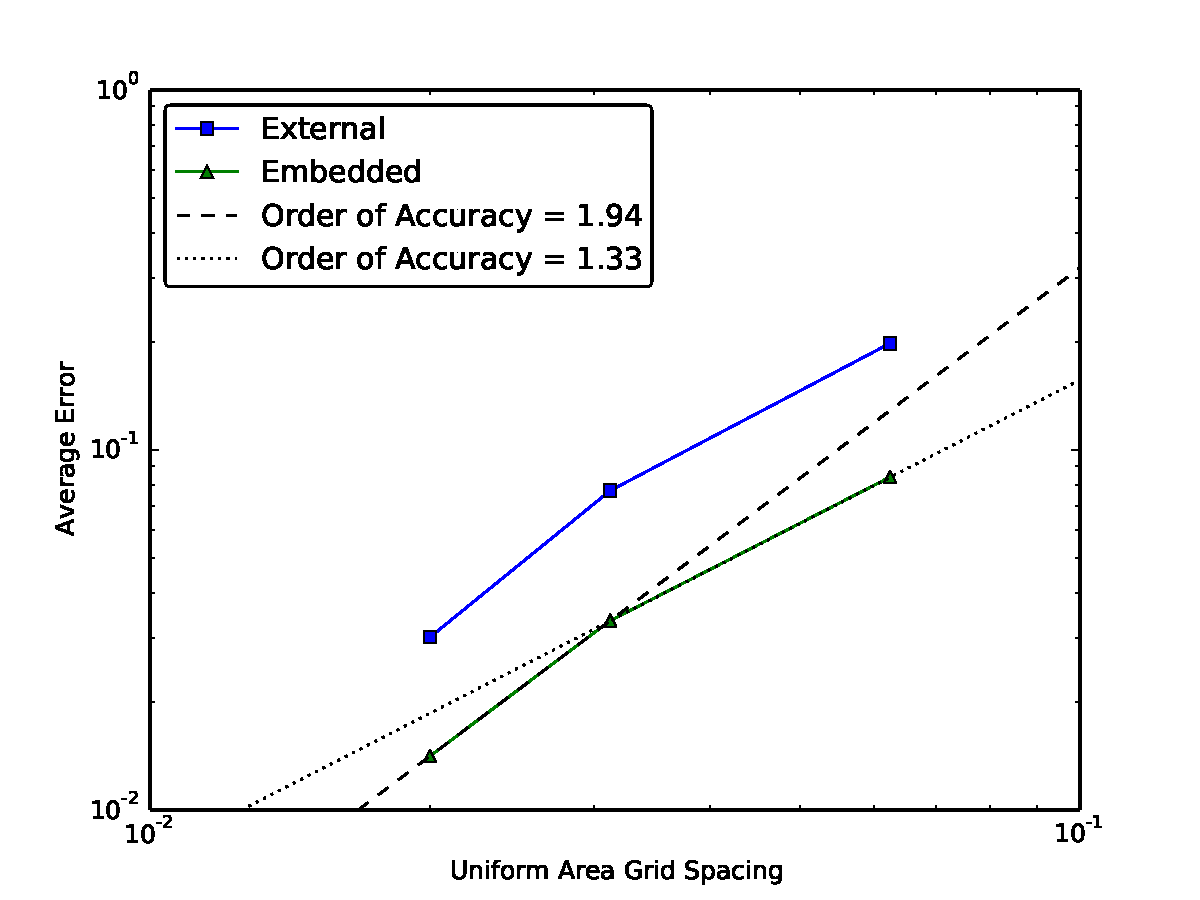
\includegraphics[width=0.5\textwidth]{error_oscflow}
	\caption{Error plotted against grid spacing shows the two solvers' order of accuracy for an oscillating cylinder in flow.}
	\label{fig:oscerror}
\end{figure}

\subsection{Performance}
Performance is evaluated by comparing the total number of cells and the computational time.
Most of these simulations are run twice on different GPUs.
The NVIDIA K20 is a dedicated computational graphics card with nearly 2500 processor cores and the NVIDIA 750 ti is a less powerful card with 640 cores.

Figure~\ref{fig:cyperf} shows the performance of an immobile impulsively started cylinder.
\begin{figure}[!htb]
	\centering
	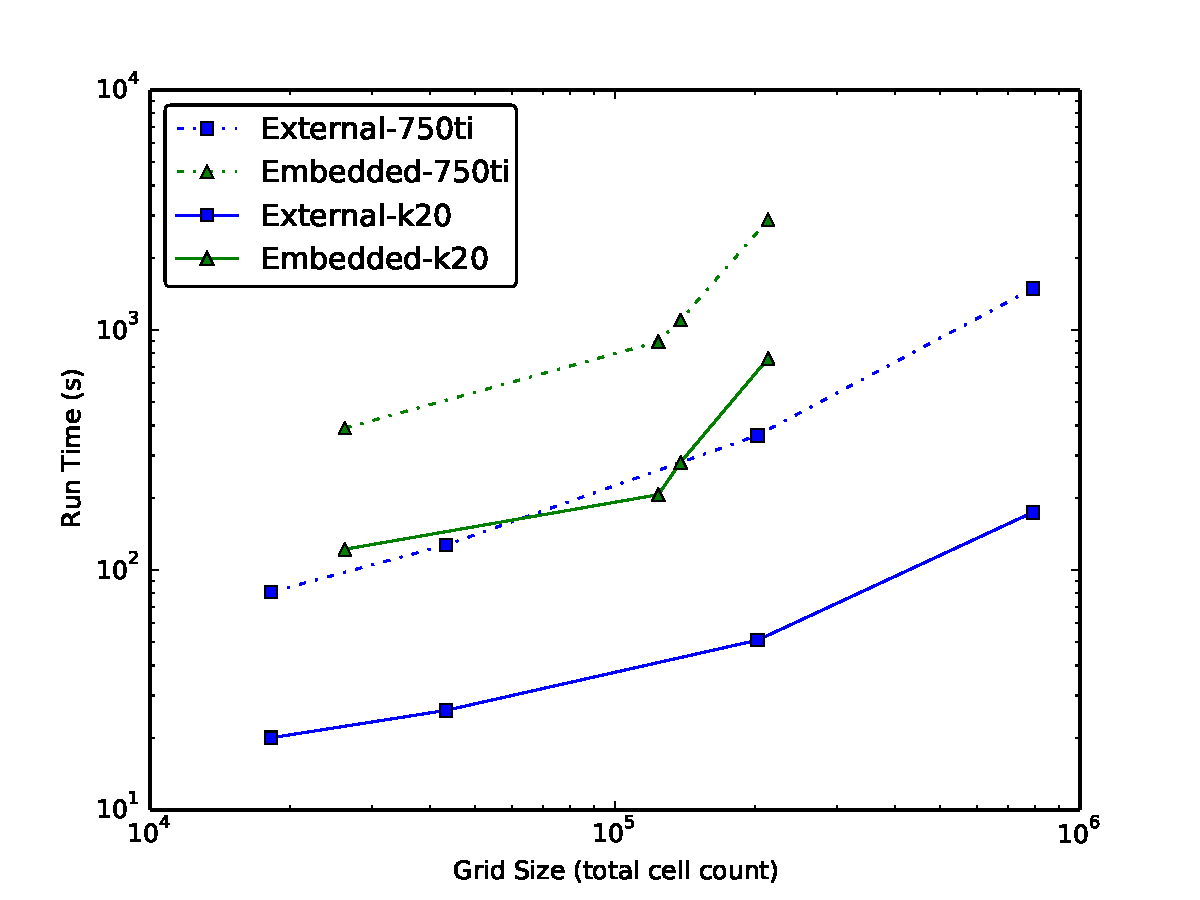
\includegraphics[width=0.5\textwidth]{cylinder_performance}
	\caption{Impulsively started cylinder performance.}
	\label{fig:cyperf}
\end{figure}
Computational time for both methods, across every type of simulation, is dominated by the Poisson equation linear algebra.
The question then becomes: why does the Poisson solver take longer for the embedded method?
Answering this question requires a look at the linear algebra multi-grid method.
The modified embedded methods use non-standard stencils near the body because it enforces boundary conditions inside the Poisson solver.
Linear algebra solvers commonly encounter tri-diagonal or banded tri-diagonal
matrices that spawn from the discretization of one-, two-, and three- dimensional Poisson equations.
As such, most linear algebra solvers are highly optimized algorithms to deal with those types of matrices.
When non-standard stencils get thrown at the solver, like those found at ghost and hybrid nodes in the embedded method, the solver is unable to efficiently solve the system of equations---resulting in more iterations and longer computational time.
The external solver ends up being much faster because it uses the standard Poisson stencil for the entire domain.

It is worth noting the difference in slope between the solvers' performance curves.
The external method is more shallow than the embedded method.
This means that means that the embedded method is scaling poorly as the cell count increases.

Figure~\ref{fig:oscperf} the performance of an impulsively started oscillating cylinder.
Similar trends to the impulsively started cylinder test can be observed here.
Most obvious is the order of magnitude difference in the time taken for each method.
In addition, the external method scales better with cell count.
Lastly, it is possible to see another effect caused by GPU scaling, which was not visible for the impulsively started cylinder.
Previously, the more powerful GPU (specifically as measured by the amount of processor cores available) achieved roughly the same speedup regardless of cell count.
For the oscillating cylinder, smaller cell counts achieve a low (negligible) speedup, which means that using a more powerful GPU for those simulations does not improve performance.
This happens when the non-parallel sections of the solver take more time than the parallel sections.
As cell count increases, the parallel portions become larger resulting in a more speedup.
\begin{figure}[!htb]
	\centering
	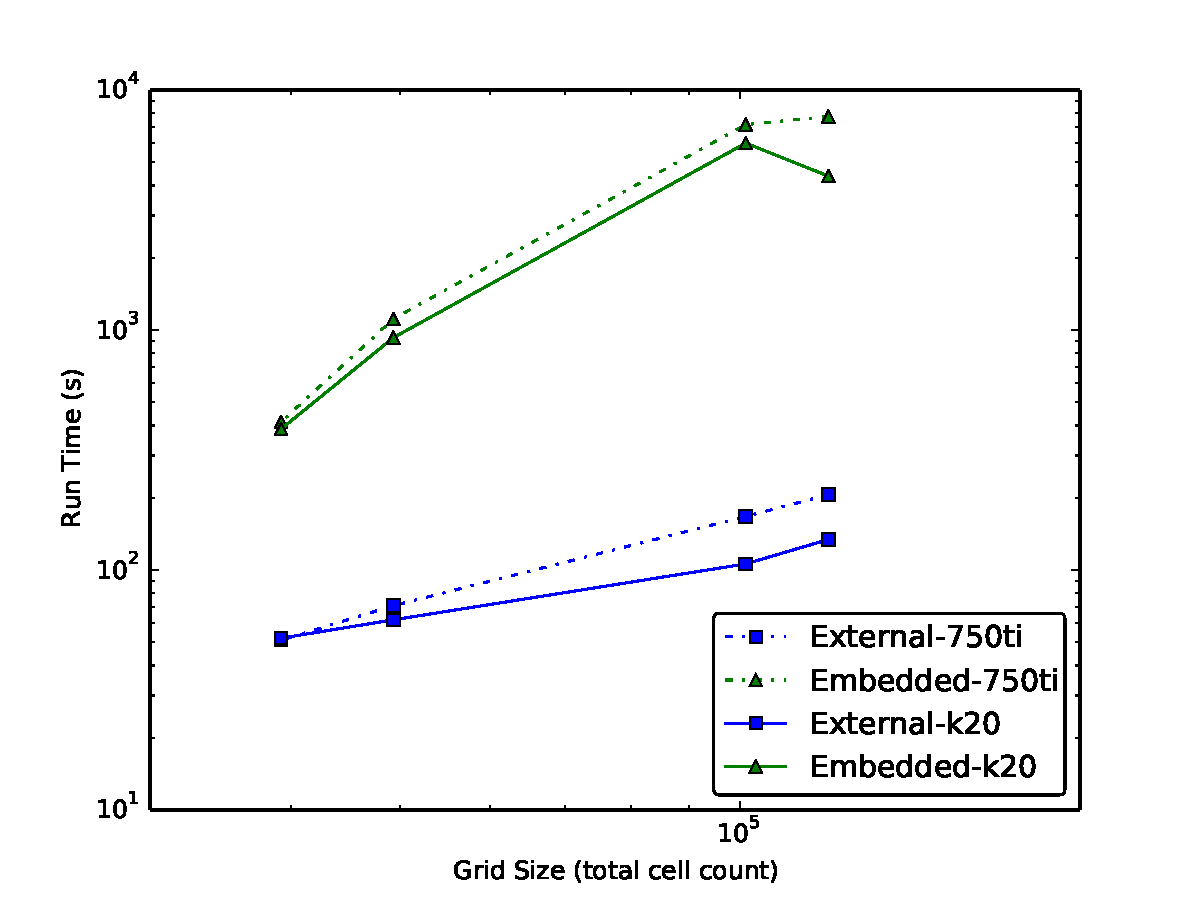
\includegraphics[width=0.5\textwidth]{osc_performance}
	\caption{Performace for flow over an in-line oscillating cylinder.}
	\label{fig:oscperf}
\end{figure}

Figure~\ref{fig:oscperf} is slightly misleading because the simulations that comprise it use the same uniform domain size and the same stretching ratios.
Total cell count is changed solely by changing the grid spacing in the uniform section.
This graph implies that the overall computational time relies on the total cell count, which is true, but the embedded method also relies on the center grid spacing h.
To verify that the computational time is dependent on center grid spacing the impulsively started oscillating cylinder simulation is run using three grid spacings of 0.0625, 0.05, and 0.03125 while keeping the overall cell count constant at $224\times224$ ($\approx$60k total) by modifying the stretch ratios.
Figure~\ref{fig:performance2} shows the resulting computational time.
Halving the grid size causes the embedded method's computational time to increase by 150\%, where the external method only increases by 33\%.
\begin{figure}[!htb]
	\centering
	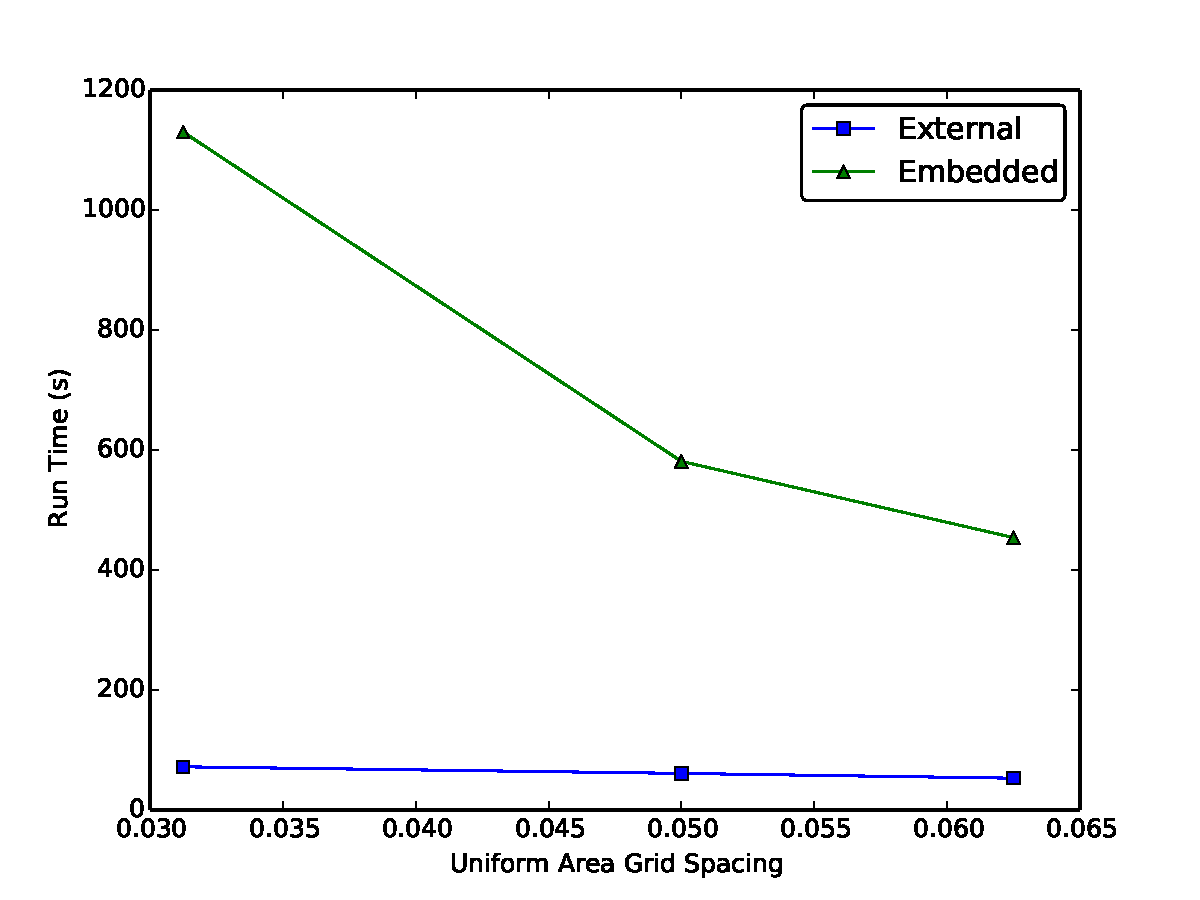
\includegraphics[width=0.5\textwidth]{performance_oscflow2}
	\caption{Computational time for flow over an in-line oscillating cylinder. The total cell count and uniform grid section size are held constant.}
	\label{fig:performance2}
\end{figure}

\section{Summary and recommendations for future work}
Immersed boundary methods are a powerful numerical approach that excel at simulating complex fluid structure interactions problems.
The study and optimization of such a device requires an accurate and fast solver.
This speed is obtained through the massive parallelism of a GPU, which is currently largely underutilized in commercial software.
cuIBM-FSI was developed to test various immersed boundary methods on a GPU, with the intent of finding the best solver to study complex freely moving body in incompressible flows.

To this end, three direct forcing immersed boundary methods were considered.
The modified Fadlun method is based off the work of Fadlun et al.~\cite{Fadlun:2000fl}.
Like the original method it does away with the force calculation at the hybrid nodes (nodes just outside the body) in favor of interpolation between the body and nearby non-hybrid fluid nodes during the intermediate velocity step.
Unlike the original Fadlun it modifies the Poisson equation to maintain mass conservation.
The external and embedded methods are based off the work of Luo et al.~\cite{Luo:2012gx}.
Both interpolate for the pressure and intermediate velocity at hybrid nodes.
They also extrapolate intermediate velocities and pressure values across the body such that hybrid node values can be calculated using a standard stencil.
These two solutions are weighted based on nodal distance from the body to suppress numerical oscillations caused by moving bodies in combination with direct forcing methods.
The external method does the weighting, interpolation, and extrapolating before and after the linear algebra solves, where the embedded method does these steps all simultaneously inside the linear algebra calculations.

The three solvers were tested using five well-studied benchmarks.
The underlying Crank--Nicholson, Adams--Bashforth, and fractional step methods used to discretize the underlying Navier--Stokes equation were tested using lid-driven cavity flow.
An impulsively started cylinder test was used to test a stationary immersed body.
This test confirmed that the original Fadlun method exhibits error in high shear situations, which led to the implementation of the modified Fadlun method.
Two simulations were used to test the methods for an imposed body motion.
Both simulations use a circular body oscillating sinusoidally on the $x$-axis.
The modified Fadlun method proved unstable with moving bodies, resulting from overwhelming numerical oscillations present in all direct forcing methods with a moving body.
Flow in the $x$-direction over the oscillating cylinder was used to qualitatively assess the numerical oscillations in the method.
This test shows that the embedded method is better at suppressing numerical oscillations than the external method.
For both methods, decreasing the grid spacing, or increasing the CFL number reduces oscillations and increases accuracy.
Oscillations in the x-direction in a static flow field is used to quantitatively verify the two methods.
This simulation showed the external method to be slightly less accurate than the embedded method, and reinforced, the previously stated results of the impulsively started oscillating cylinder simulation.

The last test is vortex-induced vibration, which features bodies that are anchored at the origin but free to move based on forces imparted by the flow.
Two methods for updating the fluid structure interaction were tested: loose and strong coupling.
All four variations of loose and strong coupling, external and embedded were able to successfully predict the forces, position, and velocity of vortex-induced vibrations.
The main difference between the embedded method and the external method is the time taken to solve each.
Each of the six simulations ($U_{red}$ one through six) is simulated to time 60.
The external loose coupling takes around eight hours where as the embedded loose coupling takes around 60.
Interestingly the strong coupling does not take much longer, with embedded strong coupling taking about 72 hours.
The main reason for this is that in each sub-step after the first, the Poisson solution has a nearly perfect field to start with which requires much less computational time.

So, which method is the ``best''?
The external method performs the best for stationary bodies, as it is the fastest while all methods produced the same results.
For moving bodies, the external method is overwhelming faster than the embedded method, and scales much better---but more prone to oscillations and slightly less accurate.
The external method is also more stable, but that seems to be mostly due to the linear algebra solver.
During optimization or parameter sweeps, it may be prudent to use the external method to narrow down the field, and then use the embedded method afterwards for more accuracy.

To improve the embedded and external methods, improving the speed of the Poisson solve is still the most efficient (and only practical) approach.
Replacing the library that cuIBM-FSI uses to solve the linear algebra, CUSP, is the first step that should be taken.
The most recent official release of CUSP was in 2014 and designed to work with CUDA 5.5.
cuIBM-FSI currently uses CUDA 7.5, and at the time of writing CUDA 8.0 is available.
Other libraries, such as AmgX are available that have more advanced multi-grid methods that may not suffer from the same scaling problems CUSP does.
In addition, CUSP does not support multiple GPUs, meaning that this code can not be used on a cluster.

\section*{Acknowledgments}
We gratefully acknowledge the support of NVIDIA Corporation with the donation of the Tesla K20 GPU used for this research.
We also thank the Barba Group for developing, maintaining, and distributing the cuIBM code.


\appendix
\setcounter{figure}{0}
% Fix for missing space between "Appendix" and letter
\renewcommand*{\thesection}{\appendixname~\Alph{section}}

%%%%%%%%%%%%%%%%%%%%%%%%%%%%%%%%%%%%%
\section{Analytical inversion of 4 \texttimes{} 4 matrix}
\label{app:inversion}
%%%%%%%%%%%%%%%%%%%%%%%%%%%%%%%%%%%%%

Given a $4 \times 4$ matrix $A$
\begin{equation}
    A =
    \begin{bmatrix}
    a_{11}&a_{12}&a_{13}&a_{14} \\
    a_{21}&a_{22}&a_{23}&a_{24} \\
    a_{31}&a_{32}&a_{33}&a_{34} \\
    a_{41}&a_{42}&a_{43}&a_{44}
    \end{bmatrix} \;,
\end{equation}
if
% \begin{gather}
%     \det{A} =
%     \begin{matrix}
%         &  &a_{11}a_{22}a_{33}a_{44}& + &a_{11}a_{23}a_{34}a_{42}& + &a_{11}a_{24}a_{32}a_{43} \\
%         &+ &a_{12}a_{21}a_{34}a_{43}& + &a_{12}a_{23}a_{31}a_{44}& + &a_{12}a_{24}a_{33}a_{41} \\
%         &+ &a_{13}a_{21}a_{32}a_{44}& + &a_{13}a_{22}a_{34}a_{41}& + &a_{13}a_{24}a_{31}a_{42} \\
%         &+ &a_{14}a_{21}a_{33}a_{42}& + &a_{14}a_{22}a_{31}a_{43}& + &a_{14}a_{23}a_{32}a_{41} \\
%         &- &a_{11}a_{22}a_{34}a_{43}& - &a_{11}a_{23}a_{32}a_{44}& - &a_{11}a_{24}a_{33}a_{42} \\
%         &- &a_{12}a_{21}a_{33}a_{44}& - &a_{12}a_{23}a_{34}a_{41}& - &a_{12}a_{24}a_{31}a_{43} \\
%         &- &a_{13}a_{21}a_{34}a_{42}& - &a_{13}a_{22}a_{31}a_{44}& - &a_{13}a_{24}a_{32}a_{41} \\
%         &- &a_{14}a_{21}a_{32}a_{43}& - &a_{14}a_{22}a_{33}a_{41}& - &a_{14}a_{23}a_{31}a_{42}
%     \end{matrix}
%     \neq 0
% \end{gather}
\begin{IEEEeqnarray}{rCl}
    \det{A} =
        &&  a_{11}a_{22}a_{33}a_{44} + a_{11}a_{23}a_{34}a_{42} + a_{11}a_{24}a_{32}a_{43} \nonumber \\
        &+& a_{12}a_{21}a_{34}a_{43} + a_{12}a_{23}a_{31}a_{44} + a_{12}a_{24}a_{33}a_{41} \nonumber \\
        &+& a_{13}a_{21}a_{32}a_{44} + a_{13}a_{22}a_{34}a_{41} + a_{13}a_{24}a_{31}a_{42} \nonumber \\
        &+& a_{14}a_{21}a_{33}a_{42} + a_{14}a_{22}a_{31}a_{43} + a_{14}a_{23}a_{32}a_{41} \nonumber \\
        &-& a_{11}a_{22}a_{34}a_{43} - a_{11}a_{23}a_{32}a_{44} - a_{11}a_{24}a_{33}a_{42} \nonumber \\
        &-& a_{12}a_{21}a_{33}a_{44} - a_{12}a_{23}a_{34}a_{41} - a_{12}a_{24}a_{31}a_{43} \nonumber \\
        &-& a_{13}a_{21}a_{34}a_{42} - a_{13}a_{22}a_{31}a_{44} - a_{13}a_{24}a_{32}a_{41} \nonumber \\
        &-& a_{14}a_{21}a_{32}a_{43} - a_{14}a_{22}a_{33}a_{41} - a_{14}a_{23}a_{31}a_{42}
    \neq 0
\end{IEEEeqnarray}
then the inverse of $A$ is
\begin{gather}
    A^{-1} = \frac{1}{\det{A}}
    \begin{bmatrix}
    b_{11}&b_{12}&b_{13}&b_{14}\\
    b_{21}&b_{22}&b_{23}&b_{24}\\
    b_{31}&b_{32}&b_{33}&b_{34}\\
    b_{41}&b_{42}&b_{43}&b_{44}
    \end{bmatrix} \;,
\end{gather}
where
\begin{align}
    b_{11} &= a_{22}a_{33}a_{44}+a_{23}a_{34}a_{42}+a_{24}a_{32}a_{43}-a_{22}a_{34}a_{43}-a_{23}a_{32}a_{44}-a_{24}a_{33}a_{42} \nonumber\\
    b_{12} &= a_{12}a_{34}a_{43}+a_{13}a_{32}a_{44}+a_{14}a_{33}a_{42}-a_{12}a_{33}a_{44}-a_{13}a_{34}a_{41}-a_{14}a_{32}a_{43} \nonumber\\
    b_{13} &= a_{12}a_{23}a_{44}+a_{13}a_{24}a_{42}+a_{14}a_{22}a_{43}-a_{12}a_{24}a_{43}-a_{13}a_{22}a_{44}-a_{14}a_{23}a_{42} \nonumber\\
    b_{14} &= a_{12}a_{24}a_{33}+a_{13}a_{22}a_{34}+a_{14}a_{23}a_{32}-a_{12}a_{23}a_{34}-a_{13}a_{24}a_{32}-a_{14}a_{22}a_{33} \nonumber\\[1ex]
    b_{21} &= a_{21}a_{34}a_{43}+a_{23}a_{31}a_{44}+a_{24}a_{33}a_{41}-a_{21}a_{33}a_{44}-a_{23}a_{34}a_{41}-a_{24}a_{31}a_{43} \nonumber\\
    b_{22} &= a_{11}a_{33}a_{44}+a_{13}a_{34}a_{41}+a_{14}a_{31}a_{43}-a_{11}a_{34}a_{43}-a_{13}a_{31}a_{44}-a_{14}a_{33}a_{41} \nonumber\\
    b_{23} &= a_{11}a_{24}a_{43}+a_{13}a_{21}a_{44}+a_{14}a_{23}a_{41}-a_{11}a_{23}a_{44}-a_{13}a_{24}a_{41}-a_{14}a_{21}a_{43} \nonumber\\
    b_{24} &= a_{11}a_{23}a_{34}+a_{13}a_{24}a_{31}+a_{14}a_{21}a_{33}-a_{11}a_{24}a_{33}-a_{13}a_{21}a_{34}-a_{14}a_{23}a_{31} \nonumber\\[1ex]
    b_{31} &= a_{21}a_{32}a_{44}+a_{22}a_{34}a_{41}+a_{24}a_{31}a_{42}-a_{21}a_{34}a_{42}-a_{22}a_{31}a_{44}-a_{24}a_{32}a_{41} \nonumber\\
    b_{32} &= a_{11}a_{34}a_{42}+a_{12}a_{31}a_{44}+a_{14}a_{32}a_{41}-a_{11}a_{32}a_{44}-a_{12}a_{34}a_{41}-a_{14}a_{31}a_{42} \nonumber\\
    b_{33} &= a_{11}a_{22}a_{44}+a_{12}a_{24}a_{41}+a_{14}a_{21}a_{42}-a_{11}a_{24}a_{42}-a_{12}a_{21}a_{44}-a_{14}a_{22}a_{41} \nonumber\\
    b_{34} &= a_{11}a_{24}a_{32}+a_{12}a_{21}a_{34}+a_{14}a_{22}a_{31}-a_{11}a_{22}a_{34}-a_{12}a_{24}a_{31}-a_{14}a_{21}a_{32} \nonumber\\[1ex]
    b_{41} &= a_{21}a_{33}a_{42}+a_{22}a_{31}a_{43}+a_{23}a_{32}a_{41}-a_{21}a_{32}a_{43}-a_{22}a_{33}a_{41}-a_{23}a_{31}a_{42} \nonumber\\
    b_{42} &= a_{11}a_{32}a_{43}+a_{12}a_{33}a_{41}+a_{13}a_{31}a_{42}-a_{11}a_{33}a_{42}-a_{12}a_{31}a_{43}-a_{13}a_{32}a_{41} \nonumber\\
    b_{43} &= a_{11}a_{23}a_{42}+a_{12}a_{21}a_{43}+a_{13}a_{22}a_{41}-a_{11}a_{22}a_{43}-a_{12}a_{23}a_{41}-a_{13}a_{21}a_{42} \nonumber\\
    b_{44} &= a_{11}a_{22}a_{33}+a_{12}a_{23}a_{31}+a_{13}a_{21}a_{32}-a_{11}a_{23}a_{32}-a_{12}a_{21}a_{33}-a_{13}a_{22}a_{31} \nonumber \;.
\end{align}

\section*{References}
\bibliography{gpu_ibm_paper}
\bibliographystyle{elsarticle-num}

\end{document}
\endinput
